%% Elsevier CAS submission, single column
%% Class and bibliography style from the Elsevier CAS bundle (cas-sc.cls, v2.4)
\documentclass[a4paper,fleqn,longmktitle]{cas-sc}

%% MiKTeX local expl3 lacks \vbox_unpack_clear:N; map it before the class loads.
\RequirePackage{expl3}
\ExplSyntaxOn
\cs_if_exist:NF \vbox_unpack_clear:N
  { \cs_new_eq:NN \vbox_unpack_clear:N \vbox_unpack_drop:N }
\ExplSyntaxOff

\usepackage[numbers]{natbib}
\usepackage{amsmath}
\usepackage{booktabs}
\usepackage{graphicx}
\usepackage{url}

%% Give the front matter block more freedom to break long lines.
\emergencystretch=3em

\shorttitle{Evaluation and verification planning under incomplete evidence}
\shortauthors{J. Zhang}

\begin{document}
\let\WriteBookmarks\relax
\def\floatpagepagefraction{1}
\def\textpagefraction{.001}

\title[mode=title]{Evaluation and verification planning for ranked environmental monitoring under incomplete evidence: VerifyRank and a methane case study}

\author[1,2]{Junjie Zhang}[orcid=0009-0004-8821-4018]
\cormark[1]
\ead{junjiezhang2024@shisu.edu.cn}
\credit{Conceptualization, Methodology, Software, Validation, Formal analysis, Investigation, Data curation, Writing -- original draft, Writing -- review and editing, Visualization}

\affiliation[1]{organization={Shanghai Academy of Global Governance and Area Studies, Shanghai International Studies University},
                city={Shanghai}, postcode={201620}, country={China}}
\affiliation[2]{organization={School of Economics and Finance, Shanghai International Studies University},
                city={Shanghai}, postcode={201620}, country={China}}

\cortext[1]{Corresponding author}

\begin{abstract}
A monitoring programme ranks a large candidate inventory every day while qualified outcome evidence exists for a fraction of it, so an analyst who must choose between two rankings ends up scoring them on the targets that carry outcomes. That practice changes the population and sets the decisive question: whether checking more archive records would settle the choice. We present VerifyRank, an evaluation layer that keeps the recommendations frozen, shares every reference outcome across policies and dates, reports the exact range of full inventory contrasts compatible with the evidence, and prices the verification that could narrow it. Applied to two airborne methane campaigns in the Permian Basin, the 2024 archive holds qualified outcomes for 1,468 of 3,921 candidate records. The paired completion range for logistic versus history spans $-0.1715$ to $0.1454$, and $0.31535$ of its $0.31688$ width comes from 2,451 records with no qualified observation, so a requested width of $0.10$ lies beyond everything archive checking can deliver. In a controlled benchmark where 632 withheld references are genuinely recoverable, the same priority order reaches a $0.10$ width after a mean of 18.3 resolved outcomes, against 206.4 for uniform checking, and greedy selection stays within a few percent of the cost constrained optimum.
\end{abstract}

\begin{highlights}
\item Rankings scored on verified targets change the population being judged
\item VerifyRank shares reference outcomes and reports the exact full inventory range
\item 99.5\% of the 2024 comparison width comes from absent qualified observations
\item The report places a 0.10 width target beyond archive checking before any spend
\item Priority order resolves 18.3 references for the same width that uniform needs 206.4 for
\end{highlights}

\begin{keywords}
incomplete evidence \sep model evaluation \sep verification planning \sep selective labels \sep monitoring priorities \sep reproducible software
\end{keywords}

\maketitle

\section{Introduction}\label{sec:intro}

A monitoring programme inspects a small number of targets each day out of a large candidate inventory, and the ranking that selects those targets is built from information available at the decision time. An analyst who must choose between two rankings turns to the archive of earlier campaigns. That archive answers unevenly, because qualified outcomes accumulate only for targets that were visited, visible to a sensor or processed successfully. The ranking covers the whole inventory while the outcome evidence covers a chosen part of it. Scoring both rankings on the covered part is standard practice, and it changes the question: the population shrinks, the rejected candidates leave the comparison, and the recommendation that would actually be deployed is no longer the one being scored. An advantage measured on the covered part can coexist with a full inventory comparison that the archive leaves wide open.

The analyst then faces a second question that is rarely asked out loud. If the archive cannot settle the choice, could more checking settle it? That question has a definite answer, and the answer is computable before any money is spent. Some unresolved records are actual observations whose endpoint was never fixed, and a reviewer can resolve them from the archive. Other candidates have no qualified observation at all, and no amount of checking will supply one, because the observation does not exist. The width that survives after every resolvable record has been returned is therefore a property of the archive rather than of the analyst's effort, and an evaluation layer can report that floor together with an ordered list of the records that would remove the resolvable part.

Environmental assessment methodology supplies the frame. Assessment quality depends on the intended use of a model, on the observations that can evaluate it and on the limits of those observations, so one performance statistic settles little on its own \citep{bennett2013}. Fit for purpose modelling treats the same judgement as the intersection of usability, reliability and feasibility, with the intended decision as the reference point \citep{hamilton2022}. For a ranked monitoring system the intended decision is a finite target budget, and the quantity of interest is the contrast that the frozen recommendations would produce across the whole inventory. A conditional score computed on verified targets answers a different question, and a confidence interval around it addresses sampling variation while saying nothing about candidates outside the reference evidence.

Selective label research showed that outcomes observed through a decision process can mislead an evaluation on the intended population \citep{lakkaraju2017}, and partial identification supplies the range of conclusions compatible with incomplete evidence \citep{manski1989}. Those lines answer the identification question. An applied archive needs three further pieces: an adapter that fixes the endpoint, the decision time and the identity of each reference; a contract that keeps the compared recommendations frozen while evidence is added; and a report that separates the verification worth paying for from evidence that no longer exists. Uncertainty analysis for deterministic models is the closest precedent for decision support under partial knowledge, because it keeps scoring rules exact while the evidence stays incomplete \citep{uusitalo2015}. Monitoring optimisation software sits on the other side of the decision and chooses measurement configurations or targets before observations exist \citep{klise2020,ravindra2024}, and an assessment layer should complement those systems rather than replace their observation models. Work on computational reproducibility supplies the vocabulary for checking whether an implementation follows its own rules \citep{essawy2020,zhu2025}, which is a narrower question than whether the archive holds enough evidence.

VerifyRank, the layer presented here, returns three quantities for one policy pair: what the verified subset says, what the full inventory comparison permits, and which unresolved records would narrow that comparison by how much. The completion arithmetic is elementary and continues existing incomplete outcome reasoning, so the contribution is the executable contract and the decision it supports. Airborne methane observation makes the problem concrete, because source activity is intermittent and repeat observation is incomplete \citep{cusworth2021,cusworth2026}. The case replays two Global Airborne Observatory campaigns in the Permian Basin against an accepted detection endpoint, with logistic regression and gradient boosting as interchangeable ranking inputs. Controlled masking of recorded outcomes supplies the known truth population used to test the verification procedures, and synthetic panels test how the layer behaves across a wide range of evidence structures.

\section{Software and methods}\label{sec:methods}

\subsection{Evidence contract}\label{sec:contract}

VerifyRank sits between a ranking system and an assessment report. An application adapter declares the candidate inventory, the decision time, the information available before that time and the rule that qualifies a future reference. The ranking system exports inclusion weights for its recommendations. Reference evidence enters a separate table once those weights are frozen, and the evaluation module scores the exported weights against the declared reference table, so an existing model can be assessed while its scoring code stays closed to future fields.

Two tables form the schema (Table~\ref{tbl:schema}). A recommendation row identifies a decision, a policy and a reference, with an inclusion weight and the target budget. Every compared policy describes the same inventory on a decision date, including zero weights. Weights lie between zero and one and sum to the budget, and fractional weights represent ties or an explicitly randomised recommendation. A reference row identifies the evidence state and, for a known outcome, carries a binary value. Cost and recovery probability fields describe declared planning scenarios rather than properties inferred from the outcome. The software rejects inconsistent budgets, duplicate keys, nonbinary resolved values and conflicting reference identities.

\begin{table}[pos=h]
\caption{Core software inputs. The endpoint and the qualification rule belong to the application adapter. Schema validation checks consistency of the supplied representation; physical validity of a label rests on the provider record.}\label{tbl:schema}
\small
\begin{tabular}{@{}p{0.20\textwidth}p{0.26\textwidth}p{0.44\textwidth}@{}}
\toprule
Input & Required information & Interpretation\\
\midrule
Recommendations & Decision, policy, reference ID, inclusion weight, budget & Complete frozen inventory, including zero weights\\
Known reference & Reference ID, positive or negative state, binary value & Outcome under the declared qualification rule\\
Ambiguous reference & Reference ID, unresolved state, resolvability & Actual observation whose endpoint remains unknown\\
Absent observation & Unique decision specific ID, absent state & No realized qualified reference; archive checking recovers nothing\\
Verification scenario & Positive relative cost; optional recovery probability & Declared planning inputs; the software infers no cost and no success rate\\
\bottomrule
\end{tabular}
\end{table}

\begin{figure}[pos=h]
  \centering
  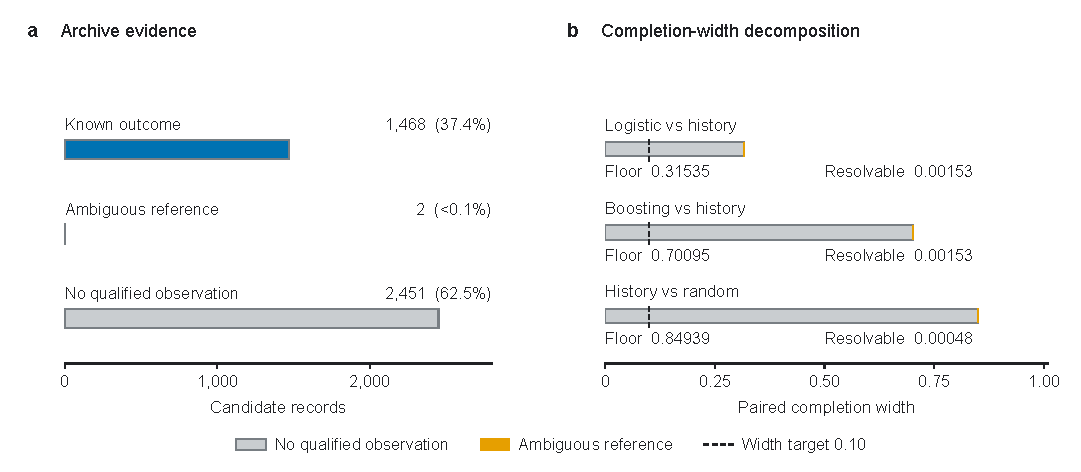
\includegraphics[width=\textwidth]{figures/Figure_1.pdf}
  \caption{Evidence state of the 2024 primary panel and the completion width it fixes. \textbf{a}, Candidate records by evidence state: 1,468 records carry a known outcome, 2 carry a qualified scene whose endpoint was never resolved, and 2,451 have no qualified observation. \textbf{b}, Paired completion width of the frozen 25\% recommendations, split by evidence state, with the requested width of 0.10 shown as a dashed line. Grey is the width contributed by records without a qualified observation, which no archive check can remove; orange is the width contributed by the single ambiguous reference, which record checking can remove. Every comparison keeps a floor far above the requested target. Widths are equal-date averages of the per-decision completion calculation.}\label{fig:evidence}
\end{figure}

An actual reference can recur across decisions, and its state and value are shared at every occurrence. A candidate without a qualified observation behaves differently, because no observation establishes that two such records carry the same outcome. Inventories and reference identities therefore come from an adapter with documented time, spatial and qualification rules. Software correctness reaches the adapter and stops there: an adapter that builds source locations from future detections, or substitutes a later and more convenient reference, produces a comparison that no downstream check can repair.

\subsection{What the comparison measures}\label{sec:measure}

Let decision \(t\) carry budget \(m_t\), and let \(w^p_{it}\) be the frozen inclusion weight of policy \(p\) for candidate \(i\). Over \(T\) equally weighted dates the policy score is the mean detection fraction of its fixed recommendations, so the contrast between policies \(a\) and \(b\) is
\begin{equation}
\Delta(y)=\frac{1}{T}\sum_t\sum_i\frac{w^a_{it}-w^b_{it}}{m_t}y_{it}
          =\sum_g C_g y_g, \qquad
C_g=\frac{1}{T}\sum_{(i,t)\in g}\frac{w^a_{it}-w^b_{it}}{m_t}.\label{eq:delta}
\end{equation}
The index \(g\) runs over one actual reference or one decision specific record without a qualified observation. Grouping precedes the range evaluation, so an unknown outcome contributes nothing when both policies select it identically, and coefficients of opposite sign cancel when they belong to the same actual reference across dates. Both properties follow from the shared identity of the reference and need no independence assumption.

Two conditional summaries stay separate. A reranked conditional score rebuilds recommendations inside the verified subset using a declared count or fraction, while a frozen conditional score keeps the original weights and divides verified selected detections by verified selected weight. The frozen version is undefined when that weight is zero, and the report labels both summaries so neither is read as a full inventory score.

For an unknown binary reference the outcome can be zero or one. With \(A\) the contribution of the known references, the exact range compatible with the evidence is
\begin{equation}
L=A+\sum_{g\,\mathrm{unknown}}\min(0,C_g),\qquad
U=A+\sum_{g\,\mathrm{unknown}}\max(0,C_g),\qquad
W=U-L=\sum_{g\,\mathrm{unknown}}|C_g|.\label{eq:range}
\end{equation}
Eq.~\eqref{eq:range} is a completion range rather than a confidence interval. Its endpoints are attainable over the declared binary completions, provided the adapter encoded every shared reference correctly. Subtracting two separately constructed policy ranges permits contradictory completions of the same shared outcomes and returns a wider answer, so the software reports both widths. It also splits the paired width into resolvable actual references, ambiguous observations and records without a qualified observation, and that split turns an uncertainty statement into a verification plan.

\subsection{Verification as an assessment decision}\label{sec:verification}

Resolving one correct binary reference removes \(|C_g|\) from the completion width whatever value it takes, so the priority order follows from the weights and consults no hidden label. Under equal cost and certain recovery, decreasing \(|C_g|\) minimises the remaining width for a fixed number of resolved records, and a reference that appears on several dates is charged once. The analyst sets a width target and a tolerance \(\epsilon\) for the policy difference; the settings used here are 0.10 and 0.02.

A current range supports one of four assessments. A lower endpoint above \(+\epsilon\) supports policy \(a\), an upper endpoint below \(-\epsilon\) supports policy \(b\), a range inside \([-\epsilon,+\epsilon]\) shows that the contrast stays inside the declared tolerance under the stated evidence assumptions, and every other case remains undetermined. Each assessment uses the current range only, so an analyst never waits for hidden truth to stop, and a complete data difference serves as a validation target in the masking experiments.

Verification is restricted to references declared recoverable. The sum of the absolute coefficients that stay unknown once those references are resolved is the attainable width floor, and when that floor exceeds the requested width no archive check can reach the target. A new observation changes the reference design and requires a new evaluation.

Under heterogeneous verification cost \(d_g>0\) the planner ranks affordable references by
\begin{equation}
\frac{|C_g|}{d_g}\quad\text{or, under a declared recovery scenario,}\quad
\frac{p_g|C_g|}{d_g},\label{eq:priority}
\end{equation}
with \(p_g\) the assumed probability of recovering a qualified binary reference. Equation~\eqref{eq:priority} states the prospective rule, in which the analyst knows the declared probability and the cost before an attempt is made. The synthetic experiments of Section~\ref{sec:regimes} also report a second benchmark that ranks by the realized product of success and coefficient once each attempt has resolved, which uses information that an analyst holds only afterwards. The two orderings are labelled separately wherever they appear. Label correctness enters as a separate assumption. With indivisible tasks and a fixed total cost the rule in Eq.~\eqref{eq:priority} is a greedy heuristic, and Section~\ref{sec:greedy} reports how far it can sit from the exact cost constrained optimum. Expected width reduction informs planning, and a realized sequence can differ because a failed attempt leaves the reference unknown. Every probability and monetary cost used below is a declared input rather than a quantity estimated from the methane archive.

Scanning the priority order under a fixed budget accepts a reference only when its whole cost fits the remaining budget, so selections at different budgets need not nest. A sequential diagnostic instead follows the priority order through successful returned labels and evaluates the updated interval after each return, and its crossing cost describes that sequence.

\subsection{Implementation, tests and reuse}\label{sec:implementation}

The generic Python package, VerifyRank version 0.2.0, runs on the Python standard library alone. Its public interface reads CSV or JSON input, validates the contract, evaluates a policy pair and prioritises unresolved references. The command line workflow writes JSON, CSV and an HTML report holding the current interval, the evidence state width, unique reference coefficients, the budget, the attainable floor and the tolerance assessment. The tutorial runs on synthetic data held in the package.

Installation, API signatures and a worked invocation appear in the software tutorial. Validation and comparison are separated from planning, so an application can supply a different cost model without touching the endpoint or the frozen recommendations. Versioned tests cover exhaustive small binary completions, shared reference cancellation, rejection of invalid input, update consistency and command line output. A Linux continuous integration workflow completes alongside a local clean installation test, and container configuration ships with the package; Docker execution remains untested. The software carries an MIT licence and ships with synthetic fixtures, while provider material and the mixed year derived panel keep their own terms; the generic software and the case archive are separate artifacts, so the tutorial runs without campaign data.

\subsection{Case study and validation design}\label{sec:case}

The case uses a 2023 Carbon Mapper catalogue snapshot and the 2024 archive associated with Cusworth et al. \citep{cusworth2026}, covering acquisitions on 16 to 24 August 2023 and 30 April to 17 May 2024. Fixed source anchors grow chronologically: an accepted detection joins the nearest existing anchor within 250 m or creates an anchor, and an anchor never moves or merges. Excluded detections discover no candidates. Source identities approximate emitting locations and carry no equipment level verification, and the observations and quality processing belong to the Carbon Mapper monitoring system \citep{duren2025}.

Daily decisions use history acquired and available before 00:00 UTC. The information scenario assumes a 24 h delay and evaluates the first geometrically and quality qualified observation within the next three days. Those timings describe archive information scenarios and make no claim about the public access conditions of the campaigns. The first qualified scene is retained even when its endpoint is ambiguous, and the endpoint is an accepted catalogue detection. A qualified nondetection records that the acceptance criterion failed under that observation, which describes detection performance and says nothing about physical zero emissions or perfect sensitivity \citep{ayasse2024}. Full geometry, scene completeness, catalogue acceptance and quality rules appear in the Supplementary Information.

The primary panel holds 3,921 candidate records across 14 decision dates, with known outcomes for 1,468 of them and two further records whose qualified scene carries no binary endpoint. The remaining 2,451 records have no qualified observation. Grouping by campaign, source and reference scene gives 3,084 macro groups, of which 632 are labelled references and 475 of those recur on more than one date. Four historical rules and two conventional learners supply ranking inputs, and the learned comparison freezes a 2023 fit before 2024 scoring with identical historical fields for every learner. The scorer rejects future reference columns, and the training rule admits a label only when its outcome was available before the fit time. Model hyperparameters, budgets and fitting guards are preserved in the Supplementary Information. The primary comparison allocates 25\% of each daily inventory with fractional treatment of ties, and conditional resampling carries complete source histories within spatial blocks, following the need to respect structured observations in evaluation \citep{roberts2017}.

Three analysis lines support the case. The first is the archive as an analyst holds it, where the width of each comparison is split into the part that record checking can remove and the part that only a new observation could remove. The second is a controlled benchmark of 200 masks in which half of the 632 labelled references are withheld and then returned in priority order, which supplies a known truth population for testing the verification procedures. The third is a synthetic regime sweep that varies the number of groups, the share of recoverable references, cost heterogeneity and recovery probability, so the behaviour of the layer can be examined outside this archive. That sweep ranks references by realized success, which supplies an upper bound on what the prospective rule of Eq.~\eqref{eq:priority} can achieve under the same conditions. Relative cost and recovery scenarios use the reference population of the case, and every scenario output is retained.

\section{Results}\label{sec:results}

\subsection{Conditional scoring reverses the answer the analyst needs}\label{sec:conditional}

The 2024 archive supplies qualified outcomes for 37.4\% of the candidate records and the 2023 archive for 53.6\%. On the verified subset the historical rate rule beats random reranked conditional precision by 0.0961, with a fixed model spatial block interval of 0.0594 to 0.1321, and logistic regression sits close to the history rule at \(-0.0102\).

For history versus random the full range runs from \(-0.3171\) to 0.5327, so a conditional advantage of 0.0961 sits beside a full inventory contrast the archive leaves open in both directions. Logistic versus history spans \(-0.1715\) to 0.1454, and boosting versus history spans \(-0.4240\) to 0.2784. Subtracting two independent policy ranges returns 1.1681 for logistic versus history, and pairing the shared outcomes returns 0.3169. The archive supports the conditional ranking result and settles no full inventory policy choice on this endpoint.

The evaluation procedure also moves the ordering. Under uniform half retention on the common defined support, original count reranking reverses the logistic versus history direction in 808 of 1,963 eligible date and mask comparisons, original fraction reranking in 478 and the frozen conditional assessment in 391, with a further 37 eligible comparisons carrying an undefined frozen conditional score. Conditional differences reach 0.1507 in the archive, which is eight times the tolerance band, so a wide completion range is not an artefact of a weak signal; the evidence simply does not reach the candidates that matter.

\subsection{The archive decides how far verification can go}\label{sec:floor}

Splitting each comparison by evidence state gives the decision that matters (Fig.~\ref{fig:evidence}, Table~\ref{tbl:decision}). For logistic versus history the paired width is 0.31688, of which 0.31535 comes from the 2,451 records without a qualified observation and 0.00153 from the single ambiguous reference. Resolving that reference removes 0.00153 at most, so 99.5\% of the width survives every check the archive permits and the attainable floor is 0.31535 against a requested width of 0.10. The same pattern holds for boosting versus history, where the floor is 0.70095 of 0.70248, and for history versus random, where the floor is 0.84939 of 0.84987.

\begin{table}[pos=h]
\caption{What an analyst can still learn from the 2024 archive. Conditional differences describe the verified subset. The paired completion range and its two components use all 14 decision dates with equal weight on the frozen 25\% recommendations. The verifiable share is the fraction of the paired width that record checking can remove.}\label{tbl:decision}
\small
\begin{tabular}{@{}p{0.22\textwidth}p{0.11\textwidth}p{0.13\textwidth}p{0.13\textwidth}p{0.13\textwidth}p{0.11\textwidth}@{}}
\toprule
Comparison & Conditional difference & Paired range & Paired width & Verifiable share & Attainable floor\\
\midrule
Logistic vs history & $-0.0102$ & $-0.1715$ to $0.1454$ & 0.31688 & 0.48\% & 0.31535\\
Boosting vs history & $-0.0474$ & $-0.4240$ to $0.2784$ & 0.70248 & 0.22\% & 0.70095\\
History vs random & $+0.0961$ & $-0.3171$ to $0.5327$ & 0.84987 & 0.06\% & 0.84939\\
\bottomrule
\end{tabular}
\end{table}

Three quantities therefore answer the analyst's question before any budget is spent: the conditional difference on the verified subset, the paired completion range, and the share of that range that verification can still touch. For all three policy pairs the third quantity is below 0.5\%, so a verification programme aimed at a width of 0.10 would spend its budget on a comparison that no record check can narrow enough. The report states that outcome explicitly and names the absent observations as the reason, which is the point at which an analyst either accepts a wider statement or commissions new measurements.

\subsection{Priority order concentrates the effort where references are recoverable}\label{sec:controlled}

The controlled benchmark returns half of the labelled references in priority order and follows the assessment after each return (Fig.~\ref{fig:value}). Decreasing the absolute coefficient reaches a width of 0.20 after a mean of 4.8 references for logistic versus history, 38.0 for boosting versus history and 79.2 for history versus random, while uniform checking needs 96.5, 203.5 and 206.0. At the target of 0.10 the same order needs 18.3, 63.1 and 143.3 references against 206.4, 260.0 and 261.3 for uniform checking, and at 0.05 it needs 34.3, 84.3 and 196.3 against 261.4, 288.3 and 288.9. Concentrating the effort therefore returns between 10 and 21 times fewer outcomes, and the advantage is largest for the comparison in which the two policies disagree most.

\begin{figure}[pos=h]
  \centering
  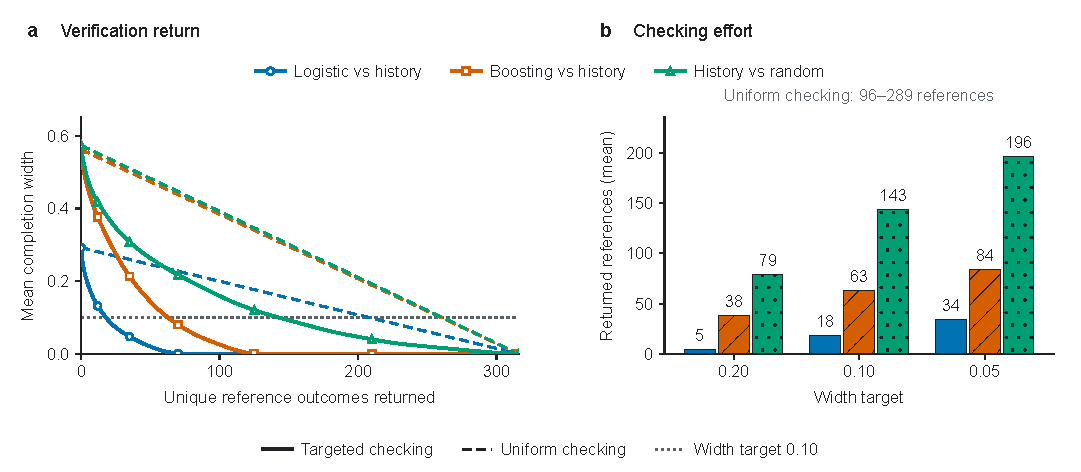
\includegraphics[width=\textwidth]{figures/Figure_2.pdf}
  \caption{What returned references buy. \textbf{a}, Mean completion width against the number of unique reference outcomes returned for the three policy pairs. Solid lines return references in decreasing order of absolute coefficient; dashed lines give the expected width of uniform fixed size revelation on the same population. The grey dashed line marks the width target of 0.10. \textbf{b}, Mean number of returned references needed to reach the width targets 0.20, 0.10 and 0.05 under the same order, with the uniform requirement of 96 to 289 references noted above the bars. Each curve and bar averages 200 masks that withhold half of the 632 labelled references.}\label{fig:value}
\end{figure}

The benchmark also fixes the limit of what verification can buy. For logistic versus history, 80 returned outcomes place the whole range inside the \(\pm0.02\) tolerance band in every one of the 200 masks, and the complete data contrast of \(-0.0140\) lies inside that band, so the honest answer is a tolerance statement. For boosting versus history, the direction becomes decidable in all 200 masks, which is consistent with the archive range crossing zero as a statement about the frozen full inventory. The controlled population and the archive answer different questions, and the report keeps both visible.

\subsection{Greedy selection stays close to the discretized optimum}\label{sec:greedy}

Equation~\eqref{eq:priority} is a heuristic once costs are indivisible, so the greedy scan was compared with a cost constrained dynamic program on the same reference population under three cost structures (Fig.~\ref{fig:greedy}). The dynamic program rounds item costs and capacity onto a 4,000 unit grid, so it returns the optimum of a discretized version of the problem and the greedy scan, which uses the original costs, can appear to beat it by a small amount where rounding is coarse. Over 41 budget levels and three policy pairs the mean relative gap is 0.44\% for logistic versus history, 0.83\% for boosting versus history and 1.71\% for history versus random. The largest single pair gap is 8.1\% and occurs at the sparsest budget, where the ordering of nearly equal ratios decides the selection. An exhaustive enumeration over 18 references with heterogeneous costs reproduces the small scale of that gap, returning 0.02894 for greedy against 0.02988 for the optimum of the same discretized problem. An analyst can therefore use the published priority order in place of a knapsack solver, and can substitute a cost constrained solver when the budget is tight and costs are indivisible.

\begin{figure}[pos=h]
  \centering
  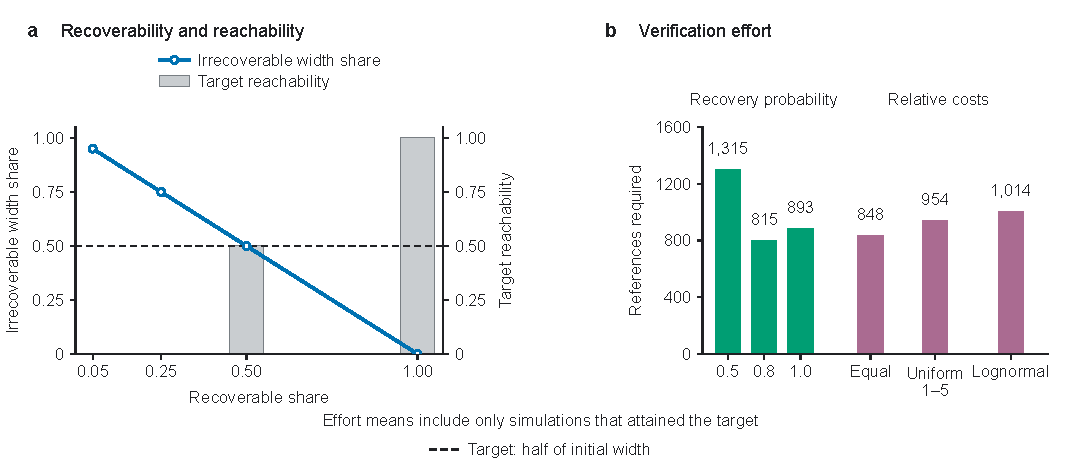
\includegraphics[width=\textwidth]{figures/Figure_4.pdf}
  \caption{What decides feasibility in synthetic regimes. \textbf{a}, Irrecoverable share of the initial width (line, left axis) and the fraction of panels whose irrecoverable floor already lies below half the initial width (bars, right axis) against the share of groups whose outcome can be recovered. This fraction records the structural feasibility of the target before any recovery attempt and is therefore larger than the fraction of panels that reach the target. The dashed line marks the target of half the initial width, and the floor exceeds that target whenever half or more of the groups stay beyond recovery. \textbf{b}, Returned references at the first attainment of half the initial width under three realized recovery shares and three cost structures, with references ranked by realized success; these bars therefore describe an upper bound for prospective planning and include only those simulations that reached the target. Each recoverable share point averages 720 panels, each recovery and cost stratum averages 960 panels, and the effort bars average between 124 and 353 successful simulations. These panels test structural behaviour of the planner and support no environmental claim.}\label{fig:regime}
\end{figure}

\subsection{Synthetic regimes locate the floor before any case study}\label{sec:regimes}

The regime sweep varies how much of the width is recoverable and how verification behaves (Fig.~\ref{fig:regime}). When 5\% or 25\% of groups are recoverable, an irrecoverable floor holds 95.0\% or 75.0\% of the initial width and no replicate reaches half the initial width, because the floor alone exceeds the target. At 50\% recoverable the target becomes reachable in 50.4\% of replicates, and at 100\% recoverable it is reachable in every replicate. The recoverable share therefore predicts feasibility almost by itself, and an analyst can test that condition on group counts and coefficients alone, without any outcome data.

\begin{figure}[pos=h]
  \centering
  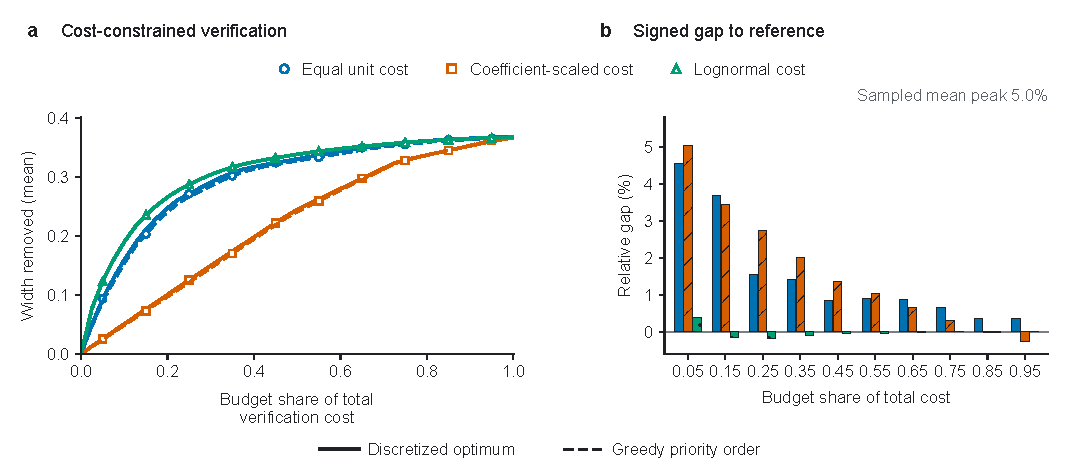
\includegraphics[width=\textwidth]{figures/Figure_3.pdf}
  \caption{Greedy priority order against the exact cost constrained optimum. \textbf{a}, Width removed against the budget share of total verification cost for the exact optimum and for the greedy rule under three cost structures. \textbf{b}, Relative gap between the greedy rule and the discretized cost constrained optimum at ten budget levels, retained with its sign so that the small negative values where rounding favours greedy remain visible. Each curve and bar averages the three policy pairs of the case over 632 recoverable references. The largest mean gap at these sampled levels is 5.0\%, and the largest gap for any single policy pair over the full budget grid is 8.1\%, which occurs at the sparsest budget.}\label{fig:greedy}
\end{figure}

Recovery probability changes the effort rather than the feasibility. Halving the width takes 1326 references at a realized recovery share of 0.5, 815 at 0.8 and 893 at 1.0, so the ordering effects of the priority rule partly offset the loss of successful returns, and the three values describe the sequence that the realized outcomes produced. Cost structure moves the effort by a smaller amount, from 848 references under equal costs to 1014 under lognormal costs, while the fraction of replicates in which the target is reachable stays near 0.38 in all three structures. The floor, not the cost model, decides whether a target can be met.

\subsection{Software verification}\label{sec:software}

The standalone package passed a clean installation test in an isolated Python 3.12.10 environment with no third party runtime dependency. CSV and JSON command line inputs produced identical numerical outputs while leaving the input files unchanged, and the synthetic and contract tests passed. Applying the package to the archived panel reproduced the macro completion ranges exactly. The generic frozen conditional output and the methane reranked conditional diagnostic remain deliberately different quantities, and the parity check keeps them apart. The analysis code, its inputs and the checksums of every source file are included in the case release, so each number in this section can be recomputed from the preserved coefficients.

\section{Discussion}\label{sec:discussion}

\subsection{What the analyst decides with the report}\label{sec:gain}

VerifyRank serves the analyst who compares monitoring recommendations against an existing archive. The analyst supplies the endpoint, the qualification protocol and the frozen target budget, and receives three answers: what the verified subset says, what the full inventory comparison permits, and which checks would change the answer. In the 2024 archive the useful decision is to withhold a full inventory superiority claim despite a favourable conditional result for history versus random, and the report shows that the single unresolved actual scene cannot narrow that comparison. Where withheld references are recoverable, as in the controlled benchmark, the same procedure returns an ordered list and updates the assessment as evidence arrives.

That decision is narrower than planning the next flight, and it arrives before a ranking system is deployed, which is where it carries value. The strongest result in the case study is negative and useful: 99.5\% of the comparison width comes from observations that do not exist, and the report says so before the verification budget is spent. An analyst who needs the conclusion has two options, both of which the report makes explicit, namely to acquire new observations under a revised protocol or to accept a wider statement about the comparison. Both are better than a verification programme that returns outcomes without moving the assessment.

Shared reference pairing matters because policy differences often sit in a small disagreement set. Much of the selected mass can be common to two policies even when neither has a narrow individual completion range, and the difference then becomes informative before either absolute score does. This property belongs to the supplied weights and reference identities. When two policies select largely different unverified candidates the paired width stays broad, and when the coefficients of one reference cancel across dates that record contributes little to the aggregate contrast however often it appears.

\subsection{Where the framework transfers}\label{sec:transfer}

The transferable object is the evaluation contract rather than the methane clustering rule or a probability model for missingness. Another application can use VerifyRank as soon as it can export the complete candidate inventory, frozen inclusion weights, a binary qualified endpoint and stable identities for repeated references. An ecological reinspection archive or a remotely sensed event catalogue can meet those requirements, and its adapter would still need independent validation of qualification, timing and identity. The synthetic sweep shows that the qualitative behaviour holds across group counts, recoverable shares, cost structures and recovery probabilities, and field performance outside the Permian campaigns stays with those adapters.

The generic implementation carries no dependency on the methane learners, the projection library or the data service. A ranking model can be a rule, a statistical learner or a multimodal system, because VerifyRank evaluates exported recommendation weights. An application with continuous mass outcomes, interacting targets, unequal environmental benefit or a travel constrained route calls for a different evaluation design, because renaming fields alone produces no valid binary equal target assessment. Bounded continuous outcomes would motivate a separate extension, and route dependent observation with policy feedback needs a different formulation.

Software practice guidance emphasises licence, versioning, documentation and verification \citep{lemmen2024}, and an audit of global impact models shows why tests and accessible code demonstrate capability while leaving scientific correctness to be established separately \citep{nyenah2024}. VerifyRank separates schema, comparison and planner, and it carries regression tests against declared cases. Its maintenance policy requires versioned schema and assessment rule changes, and that policy remains a proposed process whose community adoption is unobserved. The execution evidence available here is an internal clean environment reconstruction, which differs from third party reproduction \citep{essawy2020}.

\subsection{Costs, recovery and label quality}\label{sec:costs}

The coefficient priority answers which reference can reduce uncertainty in one fixed comparison, and it leaves the practical cost of verification to the application. An application that needs a guaranteed optimum with indivisible costs can replace the greedy heuristic with an exact cost constrained solver while keeping the same coefficients and the same evidence contract, and Section~\ref{sec:greedy} bounds what that substitution is worth on this population.

Real planning needs costs and recovery estimates from the relevant annotation or retrieval process. The primary completion range treats a known binary value as correct, and the computational metadata reconstruction checks only whether rules were implemented consistently. Where the width floor already exceeds the requested target, as it does for every comparison in this archive, incorrect supplied labels move the interval without changing that conclusion, because the floor alone decides the assessment. The label error sensitivity nevertheless remains part of the report, and it estimates no error rate from the archive.

\subsection{Case boundaries}\label{sec:boundaries}

The methane case holds two short campaigns in one basin, with some geographically overlapping source anchors and retrospective metadata. It illustrates the assessment problem, and its estimates stay inside that archive. The accepted detection endpoint depends on instrument and qualification rules, and the assumed availability delays describe archive information scenarios. The fixed replay neither changes subsequent candidate histories nor measures emissions, flight hours or repairs under an adaptive policy. These boundaries limit environmental generalisation while the finite input comparison, the software validation and the synthetic regimes stay assessable inside them.

\section{Conclusion}\label{sec:conclusion}

VerifyRank connects an incomplete evidence comparison to an explicit verification decision. It keeps recommendations frozen, shares reference outcomes across policies and dates, separates recoverable uncertainty from evidence that no longer exists, and reports the width floor that no archive check can remove. The methane case shows that a conditional ranking result can leave a full inventory policy choice open and that the archive itself fixes how far verification can go, while the controlled benchmark shows how a label free priority order concentrates the effort when withheld references are recoverable. For this archive the honest answer is that 99.5\% of the comparison width rests on observations that were never made, and the report states that conclusion before a verification budget is committed.

\section*{Data and code availability}

VerifyRank version 0.2.0 is publicly available at \url{https://github.com/williamjay1/verifyrank/releases/tag/v0.2.0}, with MIT licensed original software, tests, documentation and synthetic examples. The methane case materials, version 2026.10.06, are publicly available separately at \url{https://github.com/williamjay1/verifyrank-methane-case/releases/tag/v2026.10.06}, including derived data, reconstruction scripts, numerical outputs and source specific data terms. The MIT software licence covers the software, while provider observations and mixed year derived data keep their own terms. The Linux continuous integration run at \url{https://github.com/williamjay1/verifyrank/actions/runs/37425443624} completed successfully, which implies no third party reproduction.

The 2024 Global Airborne Observatory inputs are available in the provider archive accompanying Cusworth et al. \citep{cusworth2026}, Zenodo record 17862304, \url{https://doi.org/10.5281/zenodo.17862304}. The 2023 catalogue is a frozen Carbon Mapper service snapshot, and its retrieval and qualification are documented in the Supplementary Information. Carbon Mapper attribution and the applicable noncommercial and redistribution conditions stay with the mixed year material, while the 2024 source archive retains its stated CC BY 4.0 licence. New deposits for this software and case release remain an author action, and no DOI has been issued for these new artifacts; the provider DOI above identifies the source archive.

\section*{Declaration of AI assistance}

OpenAI Codex was used only for limited Python code assistance and English language polishing. All substantive research tasks, including study design, data collection and processing, analysis, interpretation, and manuscript preparation, were performed by the authors. AI did not generate or alter data or determine conclusions, and the authors take full responsibility for the manuscript.

\section*{Funding}

This research received no external funding.

\section*{Declaration of competing interest}

The author declares no competing financial interests or personal relationships that could have appeared to influence the work reported in this article.

\section*{Ethical statement}

The study analyses existing airborne remote sensing archives and reports no human or animal subjects, so no ethical approval was required.

\printcredits

\bibliographystyle{elsarticle-num}
\bibliography{verifyrank-refs}

\end{document}
